\begin{figure}
    \centering
    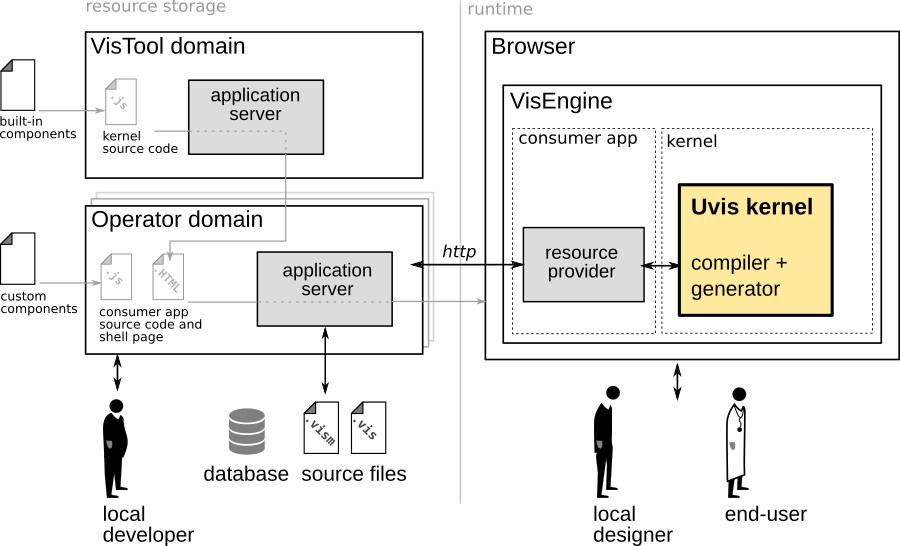
\includegraphics[width=0.9\textwidth]{images/architecture_diagram.jpg}
    \caption{System architecture for VisTool}
    \label{img:architecture}
\end{figure}

I propose hereby an architecture through which it is possible to handle the indirection in the vism file properly while offering in the same time an user experience that meets the normal expectations and habits of users (allowing to navigate naturally to a given specific vism file through the address bar of the browser).

\todo[inline]{above this paragraph the words visEngine and kernel should not be used (not introduced yet).}
The idea relies on the principle that the kernel will always be executed in combination with a domain specific application (I will refer to this application as the consumer application) that is maintained by the local developer and is shipped to the browser --thanks to the operator domain's application server-- as an HTML document (I will refer to this document as the shell page). The shell page also contains a reference to the kernel that is subsequently downloaded. Part of the domain application is the resource provider, a method that must be written by the local developer. It works as a routing mechanism that the kernel can use when it needs to find a resource on the operator domain. The resource provider should, of course, point to destinations that do actually return the expected resources. The domain specific application and the kernel together form the VisEngine. Thanks to the visEngine, the end-users can perform their activities.
\lstinputlisting[
    caption={example of a resourceProvider method},
    label={lst:resourceProvider}
]{code/resourceProvider.js}

Listing~\ref{lst:resourceProvider} shows a concrete implementation of the resource provider as it is implemented in the consumer application I will introduce very soon. The function takes a type (a string) and a resource (an object) as it's input parameters (which the kernel provides). The function immediately returns a new Promise in order to properly handle the result of the resource call that will most likely be asynchronous. The executor function within the promise shows that depending on the type, an AJAX request is opened using the data contained in the resource object and sent over to the operator domain. The kernel will be ready to use the result when the Promise will fulfill.

The role played by the resource provider is central. Since the kernel itself does not have any knowledge about the operator's domain, it is the only way it can retrieve the data it needs. It allows to decouple the kernel from the context in which it is used allowing potentially multiple domain to use simultaneously the same kernel specification (source code). The task of the kernel itself is limited to the simple task of compiling and generating the GUI within the context of use.

This architecture deserves the credit of being highlighted as the most original part of my project. It represents a new contribution that I hope to bring to the research field around VisTool~\cite{lauesen2009}~p.17. The way I deal with other parts of the project are not novel but they are equally interesting.